%======================================================================
\chapter{Algorithms}
\label{ch: Chapter4}
%======================================================================

%----------------------------------------------------------------------
\section{Robot Model}\label{sec:robotModel}
%----------------------------------------------------------------------
The robot used in this project was a differential drive mobile robot, which has two drive wheels and a caster wheel for balance. The robot turns by applying different speeds to the left and right wheels. As shown in Fig. \ref{fig:robotGeometry}, the radius of the wheels is $R$, and the distance between the wheels is $L$. The pose of the robot is given by the $x$-coordinate ($x$), the $y$-coordinate ($y$), and the orientation, ($\theta$), as shown in Fig. \ref{fig:robotPose}.
\begin{figure}
    \centering
    \begin{subfigure}{0.3\textwidth}
        \centering
        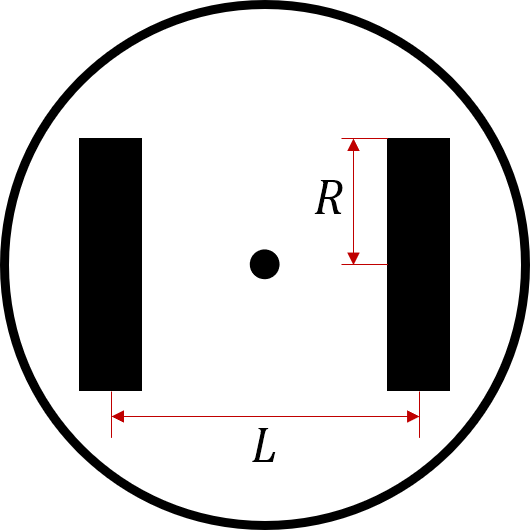
\includegraphics[width=0.9\textwidth]{figs/img/robotGeometry.png}
        \caption{Robot Geometry}
        \label{fig:robotGeometry}
    \end{subfigure}%
    \begin{subfigure}{0.7\textwidth}
        \centering
        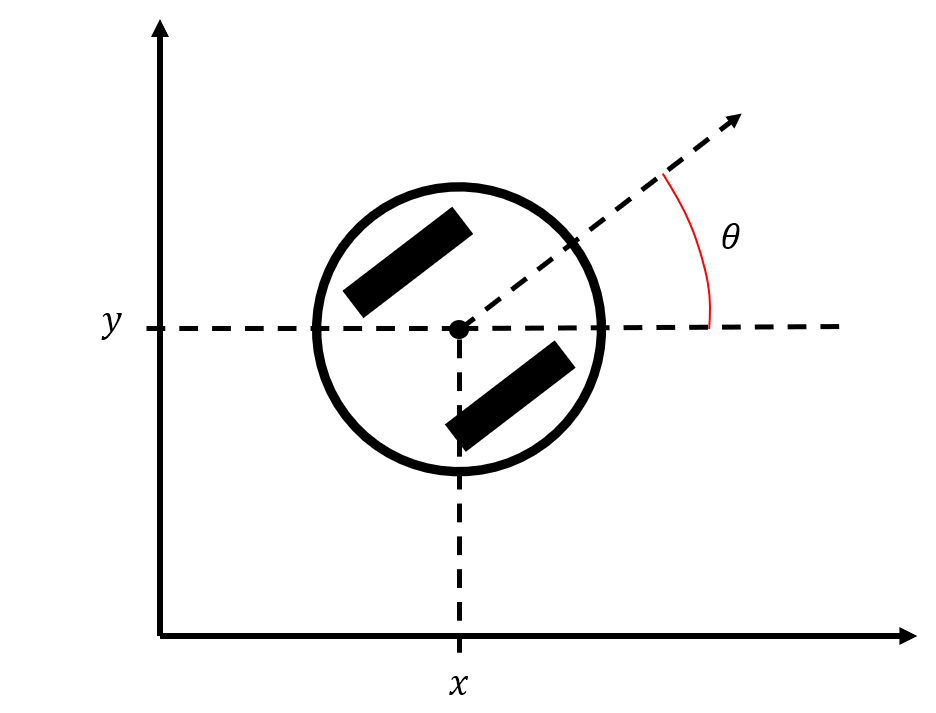
\includegraphics[width=0.9\textwidth]{figs/img/robotPose.png}
        \caption{Robot Pose}
        \label{fig:robotPose}
    \end{subfigure}
    \caption{Robot Model Parameters}
    \label{fig:robotModelParameters}
\end{figure}

\vspace*{12pt}
\noindent
Generally the robot is controlled by commanding a linear and angular speed ($v$ and $\omega$, respectively). These speeds must be converted into left and right wheel speeds. The following equations are used to calculate the angular left and right wheel speeds ($\omega_l$ and $\omega_r$, respectively):
$$\omega_l = \left(v - \omega\frac{L}{2}\right)\frac{1}{R}$$
$$\omega_r = \left(v + \omega\frac{L}{2}\right)\frac{1}{R}$$
To control DC motors in this way, the relationship between duty cycle and angular speed must be determined. Then the duty cycles to apply to the wheels can be calculated for the commanded $v$ and $\omega$.

%----------------------------------------------------------------------
\section{Localization Algorithm}
%----------------------------------------------------------------------
The localization algorithm is used to estimate the position of the remote with respect to the robot's local coordinate system. First the omnidirectional transceiver on top of the reflectors sends a signal strength request to the remote. The remote then replies with a message containing the strength of the signal it just received. This reply is detected by the receivers inside the reflectors as well as the omnidirectional transceiver. The strength detected by each of the directional receivers and the strength contained in the reply are then recorded. At this point, the entire reflector array is rotated 9\textdegree, and this process is repeated. The robot continues taking measurements in this way until the reflectors have been rotated one quarter turn. Since there are four reflectors at 90\textdegree to each other, a strength measurement has been recorded for every 9\textdegree increment around the robot. The angle of the remote is then estimated as the direction from which the strongest signal was received. The distance to the remote is calculated using the free-space path loss formula. The direction of reflector rotation is then reversed since the wires connecting the RF modules in the reflectors prevent the reflector from freely spinning. A flowchart of this algorithm is shown in Fig. \ref{fig:localizationAlgoFlowchart}.
\begin{figure}
    \centering
    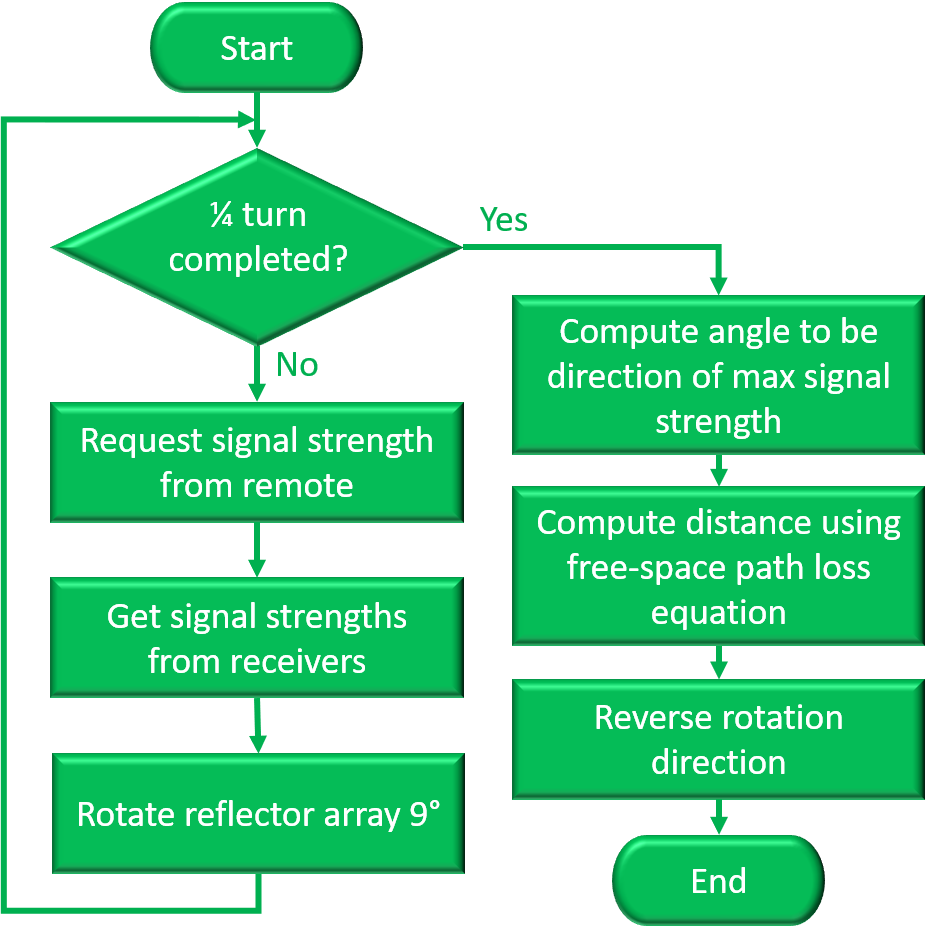
\includegraphics[width=3.5in]{figs/img/localizationAlgoFlowchart.png}
    \caption{Flowchart of Localization Algorithm}
    \label{fig:localizationAlgoFlowchart}
\end{figure}

%----------------------------------------------------------------------
\section{Navigation Algorithm}
%----------------------------------------------------------------------
The navigation algorithm is used to drive the robot toward the remote. The inputs to the navigation algorithm are the angle to the remote ($\theta_r$) and the distance to the remote ($d_r$). A target point is then calculated as the point that is in the same direction as the remote, but closer to the robot by a fixed following distance ($d_{follow}$), as shown in Fig. \ref{fig:navAlgoDiagram}. The distance to the target point is calculated as $d_{tgt} = d_r - d_{follow}$, and the angle to the target point is $\theta_{tgt} = \theta_r$. The linear and angular speeds of the robot ($v$ and $\omega$, respectively) are then calculated using proportional control by the following equations:
$$v = K_vd_{tgt}$$
$$\omega = K_\omega\theta_{tgt}$$
The appropriate duty cycles are then calculated as specified in section \ref{sec:robotModel} and applied to the wheel motors.
\begin{figure}
    \centering
    \begin{subfigure}{0.45\textwidth}
        \centering
        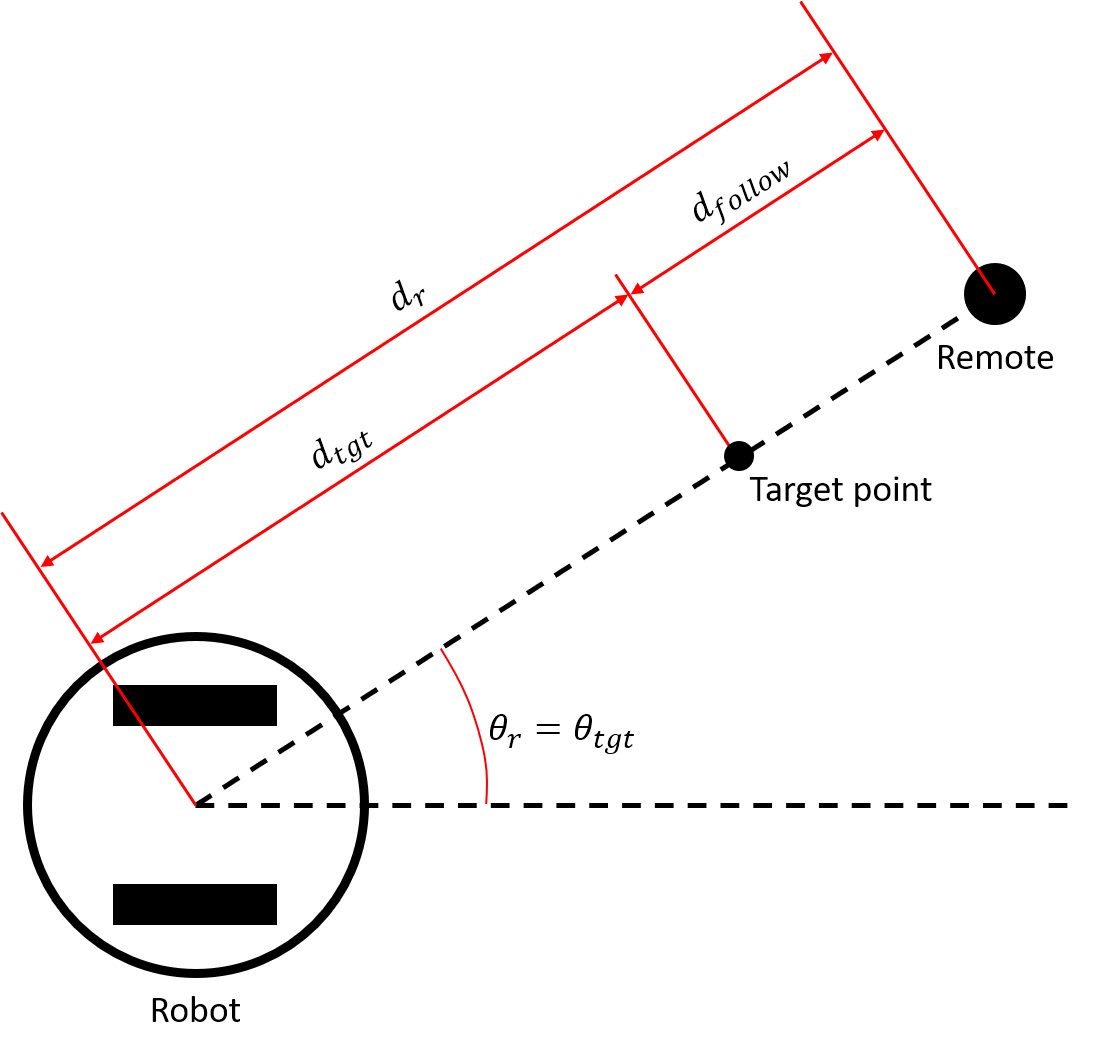
\includegraphics[width=0.95\textwidth]{figs/img/navAlgoDiagram.png}
        \caption{Target Point Diagram}
        \label{fig:navAlgoDiagram}
    \end{subfigure}%
    \begin{subfigure}{0.55\textwidth}
        \centering
        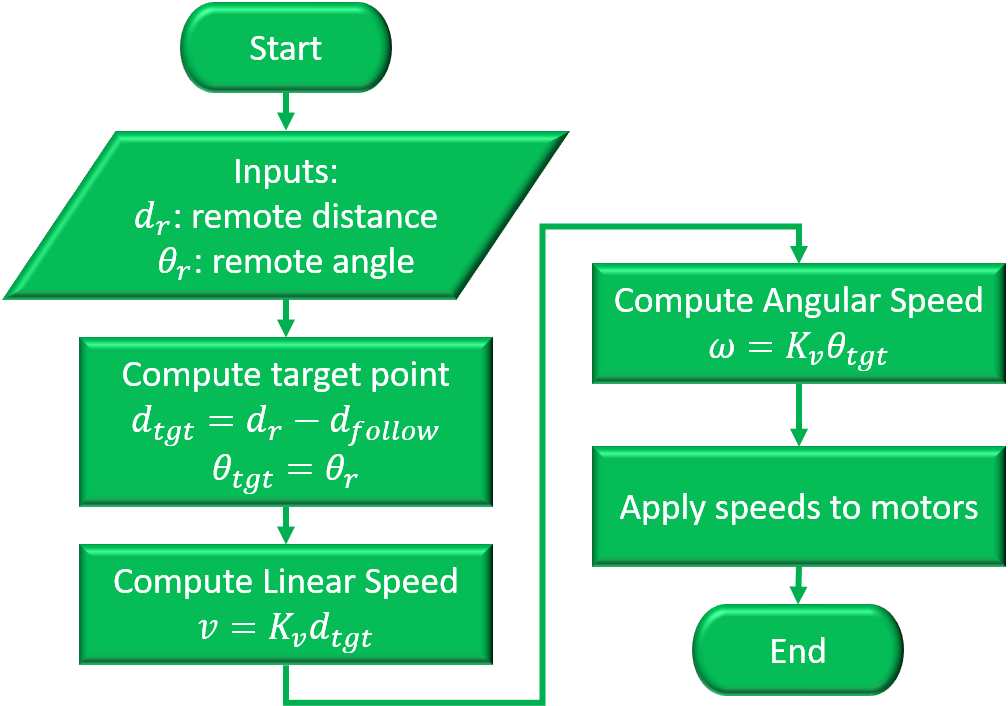
\includegraphics[width=0.95\textwidth]{figs/img/navigationAlgoFlowchart.png}
        \caption{Flowchart}
        \label{fig:navAlgoFlowchart}
    \end{subfigure}
    \caption{Navigation Algorithm Details}
    \label{fig:navAlgoDetails}
\end{figure}

%%% Local Variables:
%%% mode: latex
%%% TeX-master: "../finalReportMainV1"
%%% End: